%generare il pdf con il comando: pdflatex main.tex
\documentclass[a4paper, oneside, openany,12pt]{article}
\usepackage{graphbox}
% permette di modificare i margini
\usepackage[top=3.1cm, bottom=3.1cm, left=2.2cm, right=2.2cm]{geometry}
\usepackage{lastpage} %info sul # dell'ultima pagina del documento
\usepackage{fancyhdr} %per modificare dimensioni,margini, intestazioni e righe a piè di pagina



\fancypagestyle{plain}{
  % cancella tutti i campi di intestazione e piè di pagina
  \fancyhf{}
  
  \rhead{\sectiontitle}
  
  \rfoot{Pagina \thepage{} di \pageref{LastPage}} %es: pag: 4 di 10

  %linea orizzontale alle posizioni top e bottom della pagina
  \renewcommand{\headrulewidth}{0.2	pt}  
  \renewcommand{\footrulewidth}{0.2pt}
}
\pagestyle{plain}

%Comando Spazio
\newcommand{\Spazio}{\mbox{} \\ \mbox{} \\ }  


%\usepackage{calc} %introduce la notazione infissa per le op. aritmetiche interne a LaTeX

\usepackage[utf8]{inputenc}
\usepackage[T1]{fontenc}
\usepackage[italian]{babel} %il documento è in italiano
%\usepackage{textcomp} %The pack­age sup­ports the Text Com­pan­ion fonts, which pro­vide many text sym­bols
%(such as baht, bul­let, copy­right, mu­si­cal­note, onequar­ter, sec­tion, and yen), in the TS1 en­cod­ing.

\usepackage{graphicx}       %permette di inserire delle immagini
\usepackage{caption}        %numerazione figure e loro descrizione testuale
\usepackage{subcaption}     %sottofigure numerabili
\usepackage{float}  %permette di inserire un # qualsiasi di figure fluttuanti
\usepackage{xcolor}
\usepackage{color, colortbl}
\usepackage{rotating} %permette di ruotare le immagini
%\usepackage{changepage} %utile se c'è bisogno di aggiustare margini per centrare figure

%package utili per la math mode ( $ ... $ o \[ ... \] )
\usepackage{amsmath}
\usepackage{amssymb}
\usepackage{amsfonts}
%\usepackage{euler}    %font 'ams euler', lo stesso di 'Concrete Mathematics' di Knuth
\usepackage{amsthm}
\usepackage{mathtools}

% package utili per tabelle(\thead in particolare)
\usepackage{array, booktabs, caption}
\usepackage{makecell}
\renewcommand\theadfont{\bfseries}
\usepackage{boldline}

\usepackage{listings} %permette di inserire degli spezzoni di codice

\usepackage{tikz} %disegno di immagini vettoriali a schermo. Utile per grafi
\usetikzlibrary{arrows.meta}
\usetikzlibrary{graphs}
\usetikzlibrary{arrows}
%\usepackage{tikz-uml} %serve per disgnare l'UML, fantastica guida:
%https://perso.ensta-paristech.fr/~kielbasi/tikzuml/var/files/doc/tikzumlmanual.pdf
%download package: http://perso.ensta-paristech.fr/~kielbasi/tikzuml/

%package per le tabelle
\usepackage{booktabs} %permette di poter usare delle liste nelle tabelle
\usepackage{tabularx} 
\usepackage{longtable} %una tabella può continuare su più pagine
\usepackage{multirow} %utile per visualizzare una cella su più righe
%\usepackage{multicolumn} %cella su più colonne
%\usepackage[table]{xcolor} %rende disponibile l'utilizzo di un colore per lo sfondo
                        %delle celle di una tabella

%crea una cella per le tabelle in grado di andare a capo con \newline
%https://tex.stackexchange.com/questions/12703/how-to-create-fixed-width-table-columns-with-text-raggedright-centered-raggedlef
\usepackage{array}
\newcolumntype{L}[1]{>{\raggedright\let\newline\\\arraybackslash\hspace{0pt}}m{#1}}
\newcolumntype{C}[1]{>{\centering\let\newline\\\arraybackslash\hspace{0pt}}m{#1}}
\newcolumntype{R}[1]{>{\raggedleft\let\newline\\\arraybackslash\hspace{0pt}}m{#1}}


%indice con i puntini
\usepackage{tocloft}
\renewcommand\cftsecleader{\cftdotfill{\cftdotsep}}

%Pacchetto per i colori delle tabelle
\usepackage{color, colortbl}

%http://ctan.mirror.garr.it/mirrors/CTAN/macros/latex/contrib/appendix/appendix.pdf
\usepackage{appendix} %aggiunge dei comandi per l'appendice
\usepackage{parskip} %aiuta LaTeX a trovare il miglior stile per i page break
\setcounter{secnumdepth}{5} % numera i sottoparagrafi
\setcounter{tocdepth}{5} %aggiunge all'indice i sottoparagrafi
%\usepackage{titlesec} %\begin{paragraph} si può usare come subsubsubsection!


\usepackage{breakurl}%\url{...} può continare alla linea successiva. (si può andare a capo)

\definecolor{Maroon}{cmyk}{0, 0.87, 0.68, 0.32}
\usepackage[colorlinks=true]{hyperref}
\hypersetup{
    colorlinks=true,
    citecolor=black,
    filecolor=black,
    linkcolor=black, % colore dei link interni
    urlcolor=blue  % colore dei link interniesterni
}

%impostazioni per il codice che deve finire dentro a
%\begin{lstlisting}

\definecolor{listinggray}{gray}{0.9}
\definecolor{lbcolor}{rgb}{0.9,0.9,0.9}
\lstset{
backgroundcolor=\color{lbcolor},
    tabsize=4,    
%   rulecolor=,
    language=[GNU]C++,
    basicstyle=\scriptsize,
    upquote=true,
    aboveskip={1.5\baselineskip},
    columns=fixed,
    showstringspaces=false,
    extendedchars=true,
    inputencoding=utf8,
    breaklines=true,
    prebreak = \raisebox{0ex}[0ex][0ex]{\ensuremath{\hookleftarrow}},
    frame=single,
    numbers=left,
    showtabs=false,
    showspaces=false,
    showstringspaces=false,
    identifierstyle=\ttfamily,
    keywordstyle=\color[rgb]{0,0,1},
    commentstyle=\color[rgb]{0.026,0.112,0.095},
    stringstyle=\color[rgb]{0.627,0.126,0.941},
    numberstyle=\color[rgb]{0.205, 0.142, 0.73},
%        \lstdefinestyle{C++}{language=C++,style=numbers}’.
}
\lstset{
  backgroundcolor=\color{white},
  tabsize=4,
  language=C++,
  captionpos=b,
  tabsize=3,
  frame=lines,
  numbers=left,
  numberstyle=\tiny,
  numbersep=5pt,
  breaklines=true,
  showstringspaces=false,
  basicstyle=\footnotesize,
  identifierstyle=\color{black},
  keywordstyle=\color[rgb]{0,0,1},
  commentstyle=\color{gray},
  stringstyle=\color{red}
}
% Creazione della copertina
\newcommand{\copertina}{
  \newgeometry{top=5cm}
  
  \begin{titlepage}
  \begin{center}
 
	\begin{tikzpicture}[remember picture, overlay, scale=.5, transform shape, opacity=0.15]
		\node[anchor=center] at (current page.west){%
		\pgfimage{Stile/logo.png}};
	\end{tikzpicture}
    
  \vspace{1cm}

  \begin{Huge}
    \textbf{Corso di Algoritmi Avanzati}\\
    \vspace{20pt}  
    \textbf{Laboratorio 1:} \\
    \textbf{Minimum Spanning Tree} \\
  \end{Huge}

  \vspace{9pt}  
  
  \begin{large}
  	\today
  \end{large}	  
  
  \vspace{15pt}
  
  \vspace{15pt}

  \begin{center}
  	
  	\begin{tabular}{ c c }
		\textbf{Busin Lorenzo} & 1237580  \\
		\textbf{Tartaggia Nicolò} &   \\
		\textbf{Voinea Ciprian} & 1237294  \\
  	\end{tabular}
  	
  \end{center}

  \end{center}
  \end{titlepage}
  
  \restoregeometry
}

\newcommand{\code}[1]{\flextt{\texttt{#1}}}

\newcommand{\gl}[1]{\textit{#1}\ped{g}}

\newcommand{\sectiontitle}{}



\begin{document}
\copertina
\tableofcontents
\pagebreak

%\listoffigures
%\listoftables

% Comando per testare con le linee più grosse
\arrayrulewidth=1pt
% Colori per la tabella
\definecolor{title_row}{rgb}{0.13, 0.59, 0.95}
\definecolor{title_text}{rgb}{1, 1, 1}

% SEZIONI DEL DOCUMENTO
% qui vanno presentate in ordine di apparizione le sezioni che compongono il documento
\section{Introduzione}
Questo elaborato ha lo scopo di illustrare il lavoro svolto per il secondo homework del corso \textit{Algoritmi Avanzati}.\\
L'homework ha come obiettivo quello di confrontare tra loro gli algoritmi per il problema intrattabile chiamato "Problema del Commesso Viaggiatore" (\textit{Traveling Salesman Problem - TSP}) definito come segue: date le coordinate $x$,$y$ di $N$ punti nel piano (i vertici), e una funzione di peso $w(u,v)$ definita per tutte le coppie di punti (gli archi), trovare il ciclo semplice di peso minimo che visita tutti gli $N$ punti (ciclo hamiltoniano). La funzione peso $w(u,v)$ è definita come la distanza Euclidea o Geografica tra i punti $u$ e $v$. La soluzione ottimale consiste nell'andare a calcolare il cammino di lunghezza minima.  
\\
L'homework ha come obiettivo quello di confrontare tra loro gli algoritmi esatti e con algoritmi di approssimazione:
\begin{enumerate}
	\item \textit{Algoritmo Held-Karp} (Sez.~\ref{held_karp})
	\item \textit{Euristica costruttiva} (Sez.~\ref{constructive_heuristic})
	\item \textit{Algoritmo 2-approssimato} (Sez.~\ref{two_approx})
\end{enumerate}


Il linguaggio in cui sono stati implementati questi algoritmi è \texttt{Python}.
Abbiamo deciso di utilizzare questo al contrario di altri linguaggi come \texttt{C++} o \texttt{Java} in quanto questa scelta ci ha permesso di utilizzare i \textit{Jupyter Notebook} e di programmare utilizzando l'IDE \textit{PyCharm} oppure con \textit{Google Colab}.

Nella Sez.~\ref{risultati} sono presenti i risultati, in forma tabellare, che confrontano le performance dei tre algoritmi, calcolati sul dataset dato, contenente 13 grafi di esempio, di dimensione compresa tra $14$ e $1000$ vertici e descritti in file \texttt{.tsp}.
Sono inoltre illustrati i grafici delle performance dei vari algoritmi.

Il lavoro è stato suddiviso equamente tra i membri del gruppo nel seguente modo:
\begin{itemize}
	\item Algoritmo Held-Karp: Lorenzo Busin
	\item Euristica costruttiva: Nicolò Tartaggia
	\item Algoritmo 2-approssimato: Ciprian Voinea
\end{itemize}

Nonostante questa suddivisione tutti i membri hanno collaborato all'implementazione degli algoritmi ed effettuato una verifica finale tramite \textit{peer review} cercando di seguire una linea di sviluppo comune.
\pagebreak


\section{Algoritmo di Karger}\label{karger}

\begin{lstlisting}[mathescape=true]
Karger(G,k)
	select a vertex r $\in$ G.V to be a root vertex
	compute a MST T for G from root r using MST-PRIM(G, c, r)
	let H be a list of vertices, ordered according to when they are first visited in a preordered tree walk of T
	return the hamiltonian cycle H
	
Full contraption()
	
\end{lstlisting}	

L'algoritmo di 2-approssimazione utilizza come sottoprocedura l'algoritmo di Prim, che fornisce un MST il cui peso dà un lower bound sulla lunghezza del ciclo della soluzione ottima del TSP sul grafo dato.\\
Questo algoritmo sfrutta la disuguaglianza triangolare, ovvero dati tre nodi A, B, C, la distanza tra A e C può al massimo la distanza tra A e B sommata alla distanza tra B e C.\\
Fintanto che la funzione del costo soddisfa tale regola, viene utilizzato il minimum spanning tree per creare un ciclo con un costo che è massimo due volte il costo della soluzione ottima, per questo si dice 2-approssimato.

\subsection{Strutture dati}

	A differenza degli altri homework, per migliorare le performance dell'algoritmo in questione, abbiamo deciso di utilizzare solamente la struttura dati Graph, implementata con i seguenti campi e metodi:
	\begin{itemize}
		\item \texttt{\textbf{n\_nodes}}
		\item \texttt{\textbf{n\_edges}}
		\item \texttt{\textbf{nodes}}
		\item \texttt{\textbf{edges}}
		\item \texttt{\textbf{init}}
		\item \texttt{\textbf{addEdge}}
		\item \texttt{\textbf{buildGraph}}
	\end{itemize}
	
\subsection{Funzioni}
	
	Le funzioni ausiliarie utilizzate per calcolare la soluzione dell'algoritmo di Karger sono le seguenti:
	\begin{itemize}
		\item \texttt{\textbf{readInput}}: ;
	\end{itemize}

\subsection{Implementazione}
	
	La soluzione del problema è stata implementata nel seguente modo:
	\begin{itemize}
		\item viene costruito il grafo \texttt{g} a partire dai lista di vertici letta dal file in input;
		\item si utilizza l'algoritmo di Prim per calcolare l'MST del grafo appena creato;
		\item tale MST viene convertito, tramite l'uso della funzione \texttt{mst\_to\_tree}, in una lista che rappresenta i padri di ciascun nodo;
		\item andando a riordinare questa lista tramite la funzione \texttt{preorder}, si ottiene un ciclo hamiltoniano al quale viene appeso in coda il primo nodo, con indice 0, per chiuderlo;
		\item viene quindi calcolata la soluzione finale andando a sommare i pesi degli archi che collegano i nodi del ciclo.
	\end{itemize}
		
\subsection{Complessità}

	Per calcolare la complessità di questo algoritmo bisogna tenere in considerazione anche le operazioni che vengono svolte da Prim e, di conseguenza, quelle svolte sullo heap.\\
	La complessità totale è quindi $O(|V|^2)$, dove V indica la lista di vertici del grafo.

\pagebreak
\section{Risultati}\label{risultati}

\subsection{Tabella dei risultati}
\begin{center}
	\begin{figure}[H]
		\centering
		\hspace{-1cm}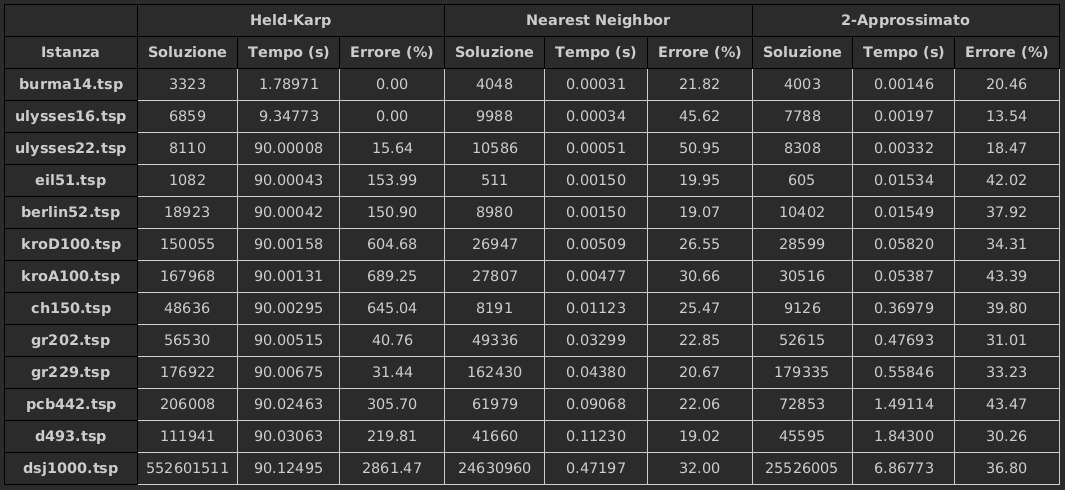
\includegraphics[width=17cm]{Img/table_results.jpg}
		\caption{Risultati del TSP calcolati}
	\end{figure}
\end{center}

\subsection{Grafico di confronto delle performance}
\begin{center}
	\begin{figure}[H]
		\centering
		\hspace{-1cm}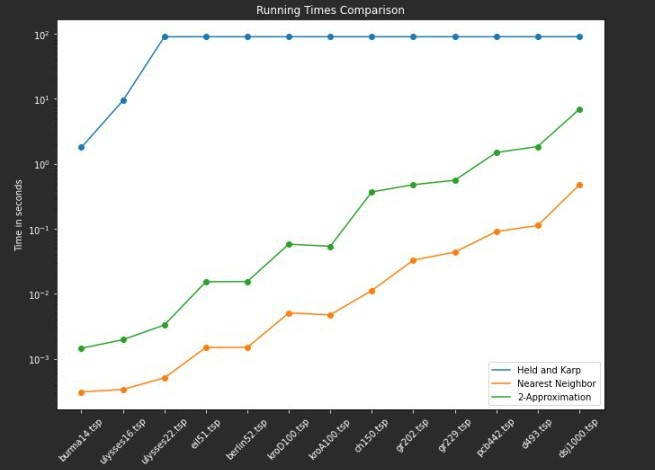
\includegraphics[width=12cm]{Img/time_graph.jpg}
		\caption{Performance degli algoritmi}
	\end{figure}
\end{center}

\subsection{Grafico di confronto degli errori}
\begin{center}
	\begin{figure}[H]
		\centering
		\hspace{-1cm}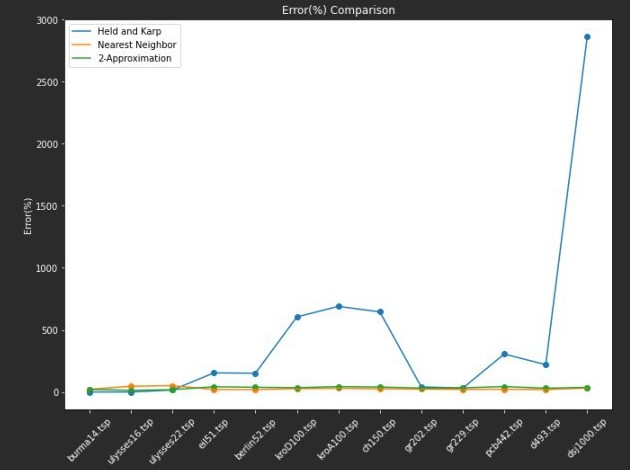
\includegraphics[width=12cm]{Img/graph_error.jpg}
		\caption{Errori degli algoritmi}
	\end{figure}
\end{center}

\subsection{Grafico di confronto degli errori con scala logaritmica}
\begin{center}
	\begin{figure}[H]
		\centering
		\hspace{-1cm}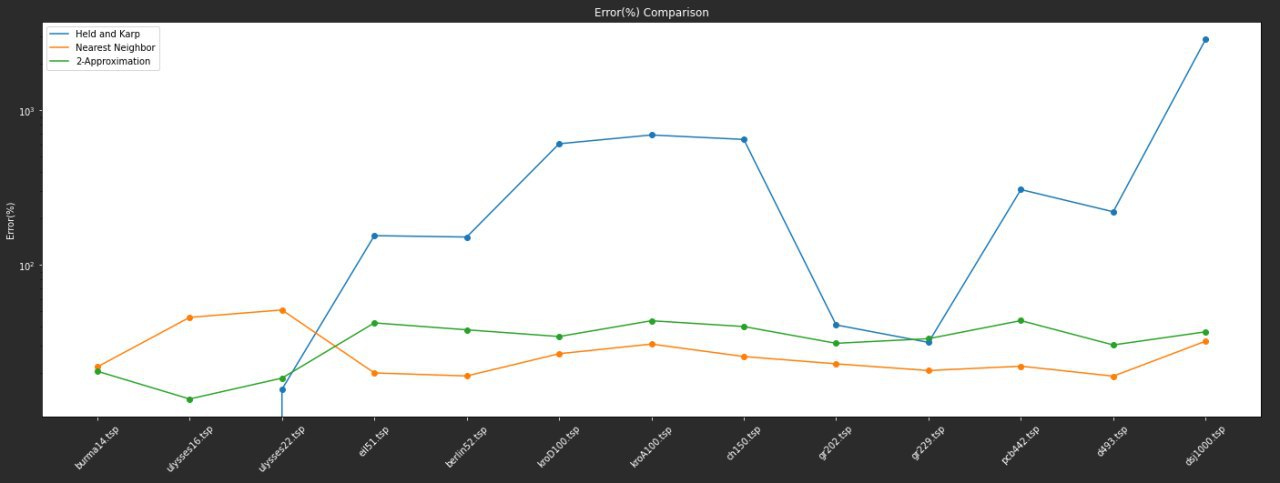
\includegraphics[width=16cm]{Img/graph_logerror.jpg}
		\caption{Logaritmo degli errori degli algoritmi}
	\end{figure}
\end{center}

	

\pagebreak
\section{Conclusione}

% Commentate i risultati che avete ottenuto: come si comportano gli algoritmi rispetti alle varie istanze? C'è un algoritmo che riesce sempre a fare meglio degli altri rispetto all'errore di approssimazione? Quale dei tre algoritmi che avete implementato è più efficiente?

Per quanto riguarda la prima e la seconda istanza, l'algoritmo di Held-Karp riesce a terminare entro il limite dei 90 secondi, trovando la soluzione ottima. 
Per quanto riguarda le altre istanze, sicuramente Held-Karp troverebbe la soluzione ottima se avessimo a disposizione un tempo infinito. 
Per le altre istanze, Nearest Neighbor risulta migliore: Held-Karp, allo scadere dei 90 secondi, ha una soluzione ottima solamente per una parte dei sottoproblemi, proseguendo poi in maniera non più ottimale. \\
Non c'è dunque un algoritmo che fa meglio degli altri in tutte le istanze dei problemi proposti, dato un limite di tempo all'algoritmo di Held-Karp.\\
Tuttavia, Nearest Neighbor è quello che presenta mediamente tempi di esecuzione ed errori inferiori rispetto agli altri algoritmi.\\
\`E stato scelto di impiegare l'algoritmo di Prim in quanto presenta una complessità minore, $O(|V|^2)$, rispetto a quello di Kruskal.
%Tra gli algoritmi di Kruskal e di Prim per il problema dell'albero di copertura minimo, è stato scelto quello di Prim poiché, essendo il grafo completo ed utilizzando l'implementazione ``ingenua'' con un vettore come coda di priorità, si ottiene una minore complessità (ovvero $O(|V|^2)$). 
Anche l'euristica Nearest Neighbor ha complessità $O(|V|^2)$, ma dai tempi rilevati si può dire che quest'ultima ha delle costanti asintotiche più basse.\\
Naturalmente l'algoritmo meno efficiente è Held-Karp che ha complessità $O(2^{|V|}*|V|^2)$, che però garantisce una soluzione ottima quando termina, ovvero avendo un tempo sufficiente.

\pagebreak


\end{document}